\documentclass[tikz,border=8pt]{standalone}
\usepackage[utf8]{inputenc}
\usepackage{amsmath,amssymb}
\usepackage{microtype}
\usetikzlibrary{arrows.meta, calc, positioning,
  decorations.pathmorphing, decorations.markings,
  shapes.geometric, patterns}

\definecolor{deepblue}{RGB}{122, 36, 53}
\definecolor{lightblue}{RGB}{234,215,218}
\definecolor{warmgold}{RGB}{154,106,31}
\definecolor{softgreen}{RGB}{124,95,88}
\definecolor{manifoldcolor}{RGB}{248,232,204}
\definecolor{distcolor}{RGB}{246,235,220}
\definecolor{midblue}{RGB}{138,90,50}

\tikzset{
  >=Stealth,
  mapsto/.style={->, line width=1.3pt, deepblue},
  pullbackarrow/.style={->, line width=1.2pt, warmgold},
  dfstyle/.style={->, line width=0.9pt, midblue, dashed},
  tanvec/.style={->, line width=1.5pt},
  mbox/.style={fill=manifoldcolor, draw=deepblue!40,
               line width=0.8pt, rounded corners=5pt, inner sep=8pt},
  pbox/.style={fill=distcolor, draw=softgreen!50,
               line width=0.8pt, rounded corners=5pt, inner sep=8pt},
}
\begin{document}
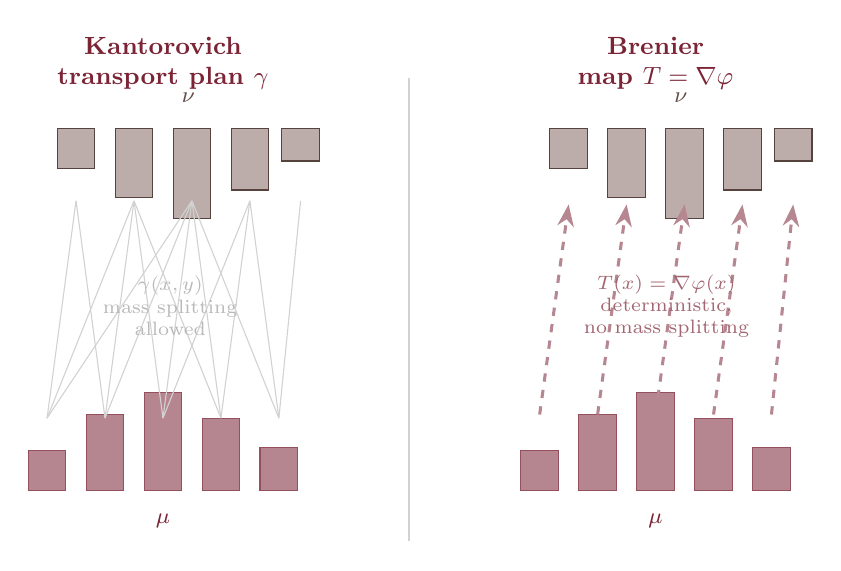
\begin{tikzpicture}[font=\small, scale=0.92]
% LEFT: Kantorovich
\begin{scope}[shift={(-3.4,0)}]
  \node[font=\small\bfseries, deepblue, align=center]
    at (0,3.4) {Kantorovich\\transport plan $\gamma$};
  \foreach \x/\h in {-1.6/0.55,-0.8/1.05,0/1.35,0.8/1.0,1.6/0.60}{
    \fill[deepblue!65,opacity=0.85]
      (\x-0.26,-2.5) rectangle (\x+0.26,-2.5+\h);
    \draw[deepblue!80](\x-0.26,-2.5)rectangle(\x+0.26,-2.5+\h);
  }
  \node[deepblue,font=\footnotesize\bfseries] at (0,-2.92) {$\mu$};
  \foreach \x/\h in {-1.2/0.55,-0.4/0.95,0.4/1.25,1.2/0.85,1.9/0.45}{
    \fill[softgreen!60,opacity=0.85]
      (\x-0.26,2.5) rectangle (\x+0.26,2.5-\h);
    \draw[softgreen!70!black](\x-0.26,2.5)rectangle(\x+0.26,2.5-\h);
  }
  \node[softgreen!80!black,font=\footnotesize\bfseries]
    at (0.35,2.92) {$\nu$};
  \foreach \xs/\xt in {
    -1.6/-1.2,-1.6/-0.4,-1.6/0.4,
    -0.8/-1.2,-0.8/-0.4,-0.8/0.4,
     0.0/-0.4, 0.0/0.4, 0.0/1.2,
     0.8/-0.4, 0.8/0.4, 0.8/1.2,
     1.6/0.4,  1.6/1.2, 1.6/1.9
  }{\draw[gray!35,thin](\xs,-1.5)--(\xt,1.5);}
  \node[gray!55,font=\scriptsize,align=center] at (0.1,0.05)
    {$\gamma(x,y)$\\mass splitting\\allowed};
\end{scope}
\draw[gray!35,thick] (0,-3.2)--(0,3.2);
% RIGHT: Brenier
\begin{scope}[shift={(3.4,0)}]
  \node[font=\small\bfseries, deepblue, align=center]
    at (0,3.4) {Brenier\\map $T=\nabla\varphi$};
  \foreach \x/\h in {-1.6/0.55,-0.8/1.05,0/1.35,0.8/1.0,1.6/0.60}{
    \fill[deepblue!65,opacity=0.85]
      (\x-0.26,-2.5) rectangle (\x+0.26,-2.5+\h);
    \draw[deepblue!80](\x-0.26,-2.5)rectangle(\x+0.26,-2.5+\h);
  }
  \node[deepblue,font=\footnotesize\bfseries] at (0,-2.92) {$\mu$};
  \foreach \x/\h in {-1.2/0.55,-0.4/0.95,0.4/1.25,1.2/0.85,1.9/0.45}{
    \fill[softgreen!60,opacity=0.85]
      (\x-0.26,2.5) rectangle (\x+0.26,2.5-\h);
    \draw[softgreen!70!black](\x-0.26,2.5)rectangle(\x+0.26,2.5-\h);
  }
  \node[softgreen!80!black,font=\footnotesize\bfseries]
    at (0.35,2.92) {$\nu$};
  \foreach \xs/\xt in {-1.6/-1.2,-0.8/-0.4,0.0/0.4,0.8/1.2,1.6/1.9}{
    \draw[->,deepblue!55, dashed, line width=1.1pt]
      (\xs,-1.45)--(\xt,1.45);
  }
  \node[deepblue!70,font=\scriptsize,align=center] at (0.15,0.05)
    {$T(x)=\nabla\varphi(x)$\\deterministic,\\no mass splitting};
\end{scope}
\end{tikzpicture}
\end{document}
